% Cluster F: the finite direct-decoration application (manuscript §10.11)
% Body-only LaTeX; preamble macros, theorem environments, and cite keys per CONVENTIONS.md.

\section{A finite direct-decoration application}\label{sec:decoration}

The certification framework of the preceding sections was assembled for a
purpose, and this final section is its intended consumer.  The setting is
the \emph{direct-decoration} configuration that the source manuscript
\cite{MWman} extracts from the decoration construction of Kahn and Lyubich
\cite{KL08}: a closed Jordan puzzle piece carrying two disjoint univalent
pullbacks of itself, iterated to produce a rooted binary tree of finite
pullback fibers accumulating on a Cantor family of end fibers.  The
resulting rooted-end compactum has \emph{infinitely many} components, so
the finite packet technology of Sections~\ref{sec:packets}
and~\ref{sec:audit} does not apply as it stands; the first task of this
section is to extend the nonseparation lemma to nested infinite packets
(Lemma~\ref{lem:nested-packets}).  The second task is geometric: the
inverse branches transport a single Jordan cell around the root continuum
into a \emph{gap-cell atlas}, a family of pairwise disjoint closed Jordan
cells, one around every finite fiber, each isolating its fiber from the
entire remaining compactum (Theorem~\ref{thm:gap-cells}).  The atlas is
precisely the dynamical realization of the cellwise criterion of
Proposition~\ref{prop:cellwise}: the cells that the cellwise certificate
asks the user to supply are here produced by the dynamics itself, at every
finite address simultaneously.  The final results assemble the package.
Packet replacement (Theorem~\ref{thm:packet-replacement}) shows that
fullifying finitely many selected fibers inside their cells preserves the
connected complement; the port lemma (Lemma~\ref{lem:impression-port})
shows that a proper compact set of protected impressions always leaves a
free port; and the protected-carrier theorem (Theorem~\ref{thm:carrier})
concludes that every finite selection of decoration addresses, decorated
with actual protected prime-end chains at the root, admits a protected
regulated connector in the sense of Theorem~\ref{thm:realization} that
avoids every unselected finite fiber and every end fiber and preserves the
transported prime ends with their cyclic order.  Throughout,
\emph{fullification} is the manuscript's term for the passage from a
compact set to its filled hull $\Fill(\,\cdot\,)$ of
Section~\ref{sec:packets}, and \emph{atom} retains the meaning fixed in
Section~\ref{sec:certificates}.

Every result of this section is reproduced, with notational streamlining
only, from Section~10.11 of the manuscript \cite{MWman}
(Lemma~10.39 through Theorem~10.45); the proofs are the manuscript's
proofs, expanded for readability.  One background result, the
direct-decoration pullback compactification (manuscript Theorem~10.37), is
\emph{quoted without proof}, and only three of its conclusions are used.
The section closes with the manuscript's own caveat on the strictly
finite, direct-scale reach of the application.

\subsection{The direct-decoration setting}\label{subsec:F-setting}

Following Section~10.11 of the manuscript \cite{MWman}, which organizes
dynamical data supplied by the decoration source of Kahn--Lyubich
\cite{KL08}, fix the following configuration.  Let $f$ be a polynomial
with
\[
K(f)=J(f),
\]
an assumption the manuscript makes explicitly, let $q\ge1$, and let $P$ be
a closed Jordan puzzle piece (in the manuscript's normalization,
$P=Y^{(n-1)q+1}$).  Put $g=f^{q}$ and let
\begin{equation}\label{eq:F-pullbacks}
g\colon Q_a\longrightarrow P,\qquad a\in\mathcal A:=\{0,1\},
\end{equation}
be the two \emph{actual univalent pullbacks} of $P$ inside $P$ (equation
(HT6) of \cite{MWman}).  Here $P$, $Q_0$, $Q_1$ are closed Jordan puzzle
pieces, the pullbacks satisfy $Q_0\cap Q_1=\varnothing$, and each proper
degree-one restriction extends to a homeomorphism of the \emph{closed}
pieces.  These closed-piece assertions---not merely disjointness of
interiors---are what the arguments below use, and the manuscript records
the separation argument for the closed pieces, which we reproduce.
Suppose $Q_0$ and $Q_1$ met at a point $z$.  Univalence of each
restriction makes $z$ a regular point of $g$, so $g$ is a local
homeomorphism at $z$; the local inverse defined on a small Jordan
half-neighborhood of $g(z)$ in $P$ would then belong to both pullback
components, contradicting their distinctness.  Hence
$Q_0\cap Q_1=\varnothing$ as closed sets, and proper degree one makes each
restriction $g\colon Q_a\to P$ a homeomorphism of closed Jordan pieces.
Write
\[
\phi_a\colon P\longrightarrow Q_a,\qquad a\in\mathcal A,
\]
for the two inverse branches; each is a homeomorphism of closed Jordan
pieces, conformal and orientation-preserving on the interior, with
$g\circ\phi_a=\id_P$.

Let $K_0\Subset\Int V_0$ be the \emph{terminal primitive root} of the
source construction: a filled Julia set, in particular a nondegenerate
full continuum.  The source construction makes $V_0$, $Q_0$, $Q_1$
distinct puzzle pieces of the common depth $nq+1$.  Their interiors are
pairwise disjoint, and $K_0$ is compactly contained in the interior of the
first; hence the \emph{root-gap relation}
\begin{equation}\label{eq:F-root-gap}
K_0\cap(Q_0\cup Q_1)=\varnothing
\end{equation}
(equation (HT7) of \cite{MWman}) holds, and the separation in
\eqref{eq:F-root-gap} is separation of \emph{closed} pieces.

\subsubsection*{Addresses, fibers, and the rooted-end compactum}
Let $\mathcal A^{<\mathbb N}$ denote the set of finite words in the
alphabet $\mathcal A=\{0,1\}$, including the empty word $\varepsilon$, and
let $\mathcal A^{\mathbb N}$ denote the set of infinite words.  For a
finite word $w=a_1\cdots a_m$ put
\begin{equation}\label{eq:F-words}
\phi_w=\phi_{a_1}\circ\cdots\circ\phi_{a_m},
\qquad
Q_w=\phi_w(P),
\qquad
K_w=\phi_w(K_0)
\end{equation}
(equation (HT8) of \cite{MWman}), with the conventions
$\phi_\varepsilon=\id_P$, $Q_\varepsilon=P$, and
$K_\varepsilon=K_0$.  For a one-letter word $a$ the cylinder $Q_a$ of
\eqref{eq:F-words} agrees with the pullback of \eqref{eq:F-pullbacks}, so
the notation is consistent; the root fiber is written $K_0$ throughout,
and the depth-one fibers are written $\phi_0(K_0)$, $\phi_1(K_0)$ with
explicit branches whenever a subscript could be misread as the root
label.  Each $\phi_w$ is a homeomorphism of $P$ onto the closed Jordan
piece $Q_w$, and $g^{|w|}\colon Q_w\to P$ is univalent.  For
$\omega\in\mathcal A^{\mathbb N}$, write $\omega|m$ for the initial
subword of length $m$ and define the \emph{end fiber}
\begin{equation}\label{eq:F-end-fiber}
E_\omega=\bigcap_{m\ge1}Q_{\omega|m}
\end{equation}
(equation (HT9) of \cite{MWman}).

Three combinatorial consequences of the standing data are used
repeatedly, and we record them once with their one-line proofs.
\emph{Nesting under extension}: appending a symbol descends one level,
\[
Q_{wa}=\phi_w\bigl(\phi_a(P)\bigr)=\phi_w(Q_a)\subset\phi_w(P)=Q_w ,
\]
so each $E_\omega$ in \eqref{eq:F-end-fiber} is a nested intersection of
nonempty compact connected sets, hence a nonempty compact connected set.
\emph{Incomparable words have disjoint cylinders}: if neither of $u,v$ is
a prefix of the other, write $u=pas$, $v=pbt$ with $p$ the longest common
prefix and $a\ne b$; then $Q_u\subset\phi_p(Q_a)$ and
$Q_v\subset\phi_p(Q_b)$, and injectivity of $\phi_p$ together with
$Q_0\cap Q_1=\varnothing$ gives $Q_u\cap Q_v=\varnothing$.
\emph{The root gap pulls back}: for every finite word $u$, applying the
injective map $\phi_u$ to \eqref{eq:F-root-gap} gives
\begin{equation}\label{eq:F-root-gap-pullback}
K_u\cap(Q_{u0}\cup Q_{u1})=\varnothing ,
\end{equation}
so every finite fiber lies in the \emph{gap} of its own cylinder, outside
both children.

The object of study is the \emph{rooted-end compactum}
\begin{equation}\label{eq:F-H}
H_\partial
=\bigcup_{w\in\mathcal A^{<\mathbb N}}K_w
\;\cup\;
\bigcup_{\omega\in\mathcal A^{\mathbb N}}E_\omega
\end{equation}
(equation (HT11) of \cite{MWman}).  We quote, as background and without
proof, the part of the manuscript's compactification theorem that the
present section uses.

\begin{theorem}[Direct-decoration pullback compactification; manuscript
Theorem 10.37, quoted background]\label{thm:F-compactification}
The set $H_\partial$ of \eqref{eq:F-H} is a compact subset of $J(f)$, and
its connected components are exactly the displayed finite pullback fibers
$K_w$ and end fibers $E_\omega$.  Moreover the transport identities
\begin{equation}\label{eq:F-transport}
g(K_{aw})=K_w,
\qquad
g(E_{a\omega})=E_\omega
\qquad(a\in\mathcal A)
\end{equation}
hold, by actual univalent branches of $f^{q}$ (equation (HT13) of
\cite{MWman}).
\end{theorem}

The proof---together with the compactness of the address space, the upper
semicontinuity of the address realization, and the careful distinction
between the geometric parent map (deleting the \emph{last} symbol), the
dynamical pre-root shift (deleting the \emph{first} symbol), and the
separate root arrow $\tau_{\mathrm{root}}$---is given in
\cite[Theorem~10.37]{MWman} and is not reproduced here; the present
section uses only the three properties displayed above.  We note for
orientation that the two deletion directions are genuinely different
maps: nesting under extension is geometric containment, while
\eqref{eq:F-transport} is dynamical transport with transition time $q$,
and the manuscript keeps them distinct.

\subsection{Fullness and nonseparation}\label{subsec:F-fullness}

The packet lemma of Section~\ref{sec:packets}
(Lemma~\ref{lem:packets}) handles finitely many pairwise disjoint full
continua.  The compactum \eqref{eq:F-H} has infinitely many components,
so an extension is needed, and the correct one is monotone: an
intersection of a decreasing sequence of finite packets does not
separate the sphere.  This is the single new topological ingredient of
the section.

\begin{lemma}[Nested finite-full-packet nonseparation; manuscript
Lemma 10.39]\label{lem:nested-packets}
Let $F_0\supset F_1\supset\cdots$ be compact subsets of the sphere
$\Chat$, each a finite union of pairwise disjoint full continua.  Then
$\bigcap_m F_m$ has connected complement in $\Chat$.  If, moreover,
$U\subset\Chat$ is a Jordan domain with $F_m\Subset U$ for every $m$, so
that each $F_m\cup(\Chat\setminus U)$ is again a finite union of pairwise
disjoint full continua, then
\[
U\setminus\bigcap_m F_m
\]
is connected.
\end{lemma}

\begin{proof}
For the first assertion, fix $m$ and let $K_1,\dots,K_N$ be the
components of $F_m$: finitely many pairwise disjoint full continua.
Lemma~\ref{lem:packets} (manuscript Lemma~10.10) shows that
$\Chat\setminus F_m$ is connected.  It is also nonempty: the finitely
many components of $F_m$ are pairwise disjoint proper closed subsets of
$\Chat$, and a connected space is not the union of two or more disjoint
nonempty closed sets, so $F_m\neq\Chat$.  Fix a point
$p\in\Chat\setminus F_0$.  Because the sets $F_m$ decrease, the open
connected complements
\[
\Chat\setminus F_0\subset\Chat\setminus F_1\subset\cdots
\]
increase, and every one of them contains the common point $p$.  A union
of connected sets sharing a point is connected, and
\[
\bigcup_m\bigl(\Chat\setminus F_m\bigr)
=\Chat\setminus\bigcap_m F_m ,
\]
so the complement of the intersection is connected, as claimed.

For the localized assertion, adjoin the exterior continuum.  Since $U$ is
a Jordan domain, the Schoenflies theorem \cite{New51} makes
$\Chat\setminus U$ a closed Jordan disk: a continuum whose complement is
the connected set $U$, hence a full continuum, and it is disjoint from
$F_m$ because $F_m\Subset U$.  Thus each
\[
F_m'=F_m\cup(\Chat\setminus U)
\]
is again a compact set that is a finite union of pairwise disjoint full
continua, and the sequence $(F_m')_m$ is decreasing.  The first assertion
applied to $(F_m')_m$ makes
\[
\Chat\setminus\bigcap_m F_m'
=\Chat\setminus\Bigl(\bigl(\textstyle\bigcap_m F_m\bigr)
\cup(\Chat\setminus U)\Bigr)
=U\setminus\bigcap_m F_m
\]
connected.
\end{proof}

With the monotone packet lemma available, fullness of every fiber and
nonseparation of the whole compactum follow from a single decreasing
approximation, which will be reused twice more in this section.

\begin{theorem}[Direct-decoration full fibers and nonseparation;
manuscript Theorem 10.40]\label{thm:full-fibers}
Every finite fiber $K_w$ and every end fiber $E_\omega$ in
Theorem~\ref{thm:F-compactification} is full.  Moreover
$\Chat\setminus H_\partial$ is connected.
\end{theorem}

\begin{proof}
\emph{Finite fibers.}
The root $K_0$ is full by the standing hypotheses of
Section~\ref{subsec:F-setting}: it is a filled Julia set, hence a
nondegenerate full continuum.  Fix a finite word $w$.  The map
$\phi_w\colon P\to Q_w$ is a homeomorphism of closed Jordan disks.  Its
boundary restriction $\partial P\to\partial Q_w$ is a homeomorphism of
Jordan curves, which by the Schoenflies theorem \cite{New51} extends to a
homeomorphism of the complementary closed disks
$\Chat\setminus\Int P\to\Chat\setminus\Int Q_w$; gluing the two
extensions along the boundary curves produces a sphere homeomorphism
$\Phi_w\colon\Chat\to\Chat$ with $\Phi_w|_P=\phi_w$, which may be taken
orientation-preserving because $\phi_w$ is orientation-preserving on
$\Int P$.  A sphere homeomorphism carries complements to complements and
connected sets to connected sets, so it preserves fullness:
$K_w=\Phi_w(K_0)$ is full.

\emph{End fibers.}
Fix $\omega\in\mathcal A^{\mathbb N}$.  By nesting under extension,
$E_\omega$ is a nested intersection of the nonempty compact connected
sets $Q_{\omega|m}$, hence a nonempty compact connected set.  Its
complement is the increasing union
\[
\Chat\setminus E_\omega
=\bigcup_{m\ge1}\bigl(\Chat\setminus Q_{\omega|m}\bigr)
\]
of connected open sets---each $Q_{\omega|m}$ is a closed Jordan
disk---all containing $\infty$.  A union of connected sets sharing a
point is connected, so $E_\omega$ is full.

\emph{The decreasing approximants.}
For $m\ge0$ define
\begin{equation}\label{eq:F-approximants}
H_m=\bigcup_{|u|<m}K_u\;\cup\;\bigcup_{|w|=m}Q_w
\end{equation}
(display (DG1) of \cite{MWman}); thus $H_0=P$ and
$H_1=K_0\cup Q_0\cup Q_1$.  We check that each $H_m$ is a finite union of
pairwise disjoint full continua.  The terms are full: the fibers $K_u$ by
the first step, the cylinders $Q_w$ because they are closed Jordan disks.
Pairwise disjointness splits into three cases, each settled by the
combinatorial facts of Section~\ref{subsec:F-setting}.
Equal-depth cylinders $Q_w,Q_{w'}$ with $w\ne w'$, $|w|=|w'|=m$ belong to
incomparable words and are disjoint.  Two distinct fibers $K_u,K_{u'}$
with $|u|,|u'|<m$: if $u$ and $u'$ are incomparable their cylinders are
disjoint, and $K_u\subset Q_u$, $K_{u'}\subset Q_{u'}$; if $u$ is a
strict prefix of $u'$, say $u'=uat$ with $a\in\mathcal A$, then
$K_{u'}\subset Q_{u'}\subset Q_{ua}$, while the pulled-back root gap
\eqref{eq:F-root-gap-pullback} keeps $K_u$ outside the child $Q_{ua}$.
A fiber $K_u$ with $|u|<m$ against a cylinder $Q_w$ with $|w|=m$: the
words are distinct since $|u|<|w|$; if incomparable, the cylinders
containing them are disjoint; if $u$ is a strict prefix of $w$, say
$w=uat'$, then $Q_w\subset Q_{ua}$ and \eqref{eq:F-root-gap-pullback}
again separates.  (The case $w$ a prefix of $u$ cannot occur, as
$|w|>|u|$.)

\emph{The approximants decrease to $H_\partial$.}
$H_{m+1}\subset H_m$: a fiber term $K_u$ of $H_{m+1}$ with $|u|<m$ is a
term of $H_m$, and one with $|u|=m$ satisfies $K_u\subset Q_u$, a term of
$H_m$; a cylinder term $Q_w$ of $H_{m+1}$ with $|w|=m+1$ satisfies
$Q_w\subset Q_{w|m}$, a term of $H_m$.  Next,
$H_\partial\subset\bigcap_mH_m$: for each $m$, a fiber $K_w$ with
$|w|<m$ is a term of $H_m$; one with $|w|\ge m$ lies in
$Q_w\subset Q_{w|m}$; and every end fiber satisfies
$E_\omega\subset Q_{\omega|m}$.  Conversely let
$x\in\bigcap_mH_m$ and suppose $x$ lies in no finite fiber.  Then for
every $m$ the membership $x\in H_m$ forces $x\in Q_{w_m}$ for some word
$w_m$ of length $m$.  Equal-depth cylinders are pairwise disjoint, and
$x\in Q_{w_{m+1}}\subset Q_{w_{m+1}|m}$, so $w_{m+1}|m=w_m$ for every
$m$: the words are coherent truncations of one unique infinite address
$\omega$ with $\omega|m=w_m$, and $x\in\bigcap_mQ_{\omega|m}=E_\omega$.
Outside the explicit finite fibers, a point of every approximant thus
determines one unique compatible infinite cylinder address, and
\[
\bigcap_m H_m=H_\partial .
\]

\emph{Conclusion.}
The sets \eqref{eq:F-approximants} form a decreasing sequence of compact
sets, each a finite union of pairwise disjoint full continua, with
intersection $H_\partial$.  Lemma~\ref{lem:nested-packets} shows that
$\Chat\setminus H_\partial$ is connected.
\end{proof}

\subsection{The gap-cell atlas}\label{subsec:F-atlas}

The next step localizes each finite fiber inside a closed Jordan cell
that isolates it from everything else in the compactum.  The cell is
produced once, at the root, by a classical uniformization argument, and
then transported everywhere by the inverse branches.

\begin{lemma}[Full-continuum Jordan neighborhood; manuscript
Lemma 10.41]\label{lem:jordan-nbhd}
If a nondegenerate full continuum $K$ is compactly contained in an open
set $G$, there is a closed Jordan disk $D$ such that
\begin{equation}\label{eq:F-jordan-cell}
K\subset\Int D\subset D\Subset G
\end{equation}
(display (DG2) of \cite{MWman}).
\end{lemma}

\begin{proof}
The complement $\Chat\setminus K$ is a simply connected domain containing
$\infty$, and $K$ is nondegenerate, so the domain is conformally a
round-disk exterior: there is a conformal homeomorphism
\[
\psi\colon\{|z|>1\}\longrightarrow\Chat\setminus K
\]
with $\psi(\infty)=\infty$ \cite{Pom92}.  For $R>1$ the image
$\psi(\{|z|=R\})$ of the round circle is an analytic Jordan curve, and we
let $D_R$ be its \emph{filled interior}, the closure of the bounded
complementary component:
\[
D_R=\Chat\setminus\psi\bigl(\{|z|>R\}\bigr).
\]
Each $D_R$ is a closed Jordan disk containing $K$ in its interior, and
the family decreases as $R\downarrow1$: for $1<R'<R$ the annulus image
$\psi(\{R'<|z|\le R\})$ lies in $D_{R}\setminus D_{R'}$, giving
$D_{R'}\subset\Int D_R$.  Moreover $\bigcap_{R>1}D_R=K$: a point of
$\Chat\setminus K$ is $\psi(z)$ for a unique $|z|>1$ and lies outside
$D_R$ for every $R<|z|$.

Suppose no $D_R$ were compactly contained in $G$.  Then for every $R>1$
the compact set $D_R\cap(\Chat\setminus G)$ would be nonempty; these
compacta decrease with $R$, so their total intersection
\[
\bigcap_{R>1}\bigl(D_R\cap(\Chat\setminus G)\bigr)
=K\cap(\Chat\setminus G)
\]
would be nonempty, contradicting $K\Subset G$.  Hence some $D=D_R$
satisfies \eqref{eq:F-jordan-cell}.
\end{proof}

Now let $G_0$ be the component of $\Int P\setminus(Q_0\cup Q_1)$
containing $K_0$.  The root-gap relation \eqref{eq:F-root-gap}, together
with $K_0\Subset\Int V_0\subset\Int P$, makes $K_0$ a compact connected
subset of the open set $\Int P\setminus(Q_0\cup Q_1)$ with positive
distance to its complement, so $K_0\Subset G_0$.  Choose a closed Jordan
disk $D$ for $K=K_0$ and $G=G_0$ by Lemma~\ref{lem:jordan-nbhd}, and
transport it through every inverse branch:
\[
D_w=\phi_w(D),\qquad w\in\mathcal A^{<\mathbb N},
\]
with $D_\varepsilon=D$.  These are the \emph{gap cells}, and the family
is the \emph{gap-cell atlas} of the decoration data; see
Figure~\ref{fig:cells}.

\begin{theorem}[Direct-decoration gap-cell atlas; manuscript
Theorem 10.42]\label{thm:gap-cells}
The closed Jordan cells $D_w$, $w\in\mathcal A^{<\mathbb N}$, are
pairwise disjoint, including for ancestor--descendant pairs of words, and
satisfy
\begin{equation}\label{eq:F-cell-position}
K_w\subset\Int D_w,
\qquad
D_w\Subset\Int Q_w\setminus(Q_{w0}\cup Q_{w1}),
\end{equation}
\begin{equation}\label{eq:F-cell-isolation}
D_w\cap H_\partial=K_w,
\qquad
g(D_{aw})=D_w
\end{equation}
(displays (DG3) and (DG4) of \cite{MWman}).  If
$S_w\Subset\Int D_w$ is compact and connected, then
\begin{equation}\label{eq:F-cell-fill}
\Fill(S_w)\Subset\Int D_w
\end{equation}
(display (DG5) of \cite{MWman}).
\end{theorem}

\begin{proof}
\emph{Position \eqref{eq:F-cell-position}.}
At the root, $K_0\subset\Int D$ and
$D\Subset G_0\subset\Int P\setminus(Q_0\cup Q_1)$ by construction.  The
map $\phi_w$ is a homeomorphism of the closed Jordan piece $P$ onto the
closed Jordan piece $Q_w$ carrying $\Int P$ onto $\Int Q_w$ and carrying
$Q_a$ onto $Q_{wa}$ for $a\in\mathcal A$.  Applying $\phi_w$ to the root
inclusions gives
$K_w=\phi_w(K_0)\subset\phi_w(\Int D)=\Int D_w$ (the sphere extension
$\Phi_w$ of the proof of Theorem~\ref{thm:full-fibers} carries the open
disk $\Int D$ onto the open disk $\Int D_w$) and
\[
D_w=\phi_w(D)
\Subset\phi_w\bigl(\Int P\setminus(Q_0\cup Q_1)\bigr)
=\Int Q_w\setminus(Q_{w0}\cup Q_{w1}).
\]

\emph{Pairwise disjointness.}
Let $u\ne v$ be finite words.  If $u$ and $v$ are incomparable, their
cylinders are disjoint and $D_u\subset Q_u$, $D_v\subset Q_v$.  If $v$ is
a strict descendant of $u$, write $v=uat$ with $a\in\mathcal A$ and $t$ a
(possibly empty) word.  Then
\[
D_v\subset Q_v\subset Q_{ua},
\]
the child of $Q_u$ with label $a$, while by
\eqref{eq:F-cell-position} the cell $D_u$ lies outside both children
$Q_{u0}\cup Q_{u1}$ of $Q_u$.  Hence $D_u\cap D_v=\varnothing$.  This
dichotomy---incomparable words are separated by their cylinders,
comparable words by the gap position of the ancestor cell---proves
disjointness for every pair.

\emph{Isolation: the first identity of \eqref{eq:F-cell-isolation}.}
The inclusion $K_w\subset D_w\cap H_\partial$ holds by
\eqref{eq:F-cell-position}.  For the converse we show that every
component of $H_\partial$ other than $K_w$ misses $D_w$; by
Theorem~\ref{thm:F-compactification} those components are the finite
fibers $K_u$, $u\ne w$, and the end fibers $E_\omega$.  The same
dichotomy applies.  If $u$ and $w$ are incomparable, then
$K_u\subset Q_u$ and $D_w\subset Q_w$ lie in disjoint cylinders.  If $u$
is a strict prefix of $w$, say $w=uat'$, then $D_w\subset Q_w\subset
Q_{ua}$ while \eqref{eq:F-root-gap-pullback} keeps $K_u$ outside
$Q_{ua}$.  If $w$ is a strict prefix of $u$, say $u=wat$, then
$K_u\subset Q_u\subset Q_{wa}$, while $D_w$ misses both children of
$Q_w$ by \eqref{eq:F-cell-position}.  For an end fiber $E_\omega$: if $w$
is a prefix of $\omega$, then
$E_\omega\subset Q_{\omega|(|w|+1)}=Q_{wa}$ for the symbol
$a=\omega_{|w|+1}$, a child of $Q_w$, which $D_w$ misses; if $w$ is not a
prefix of $\omega$, let $m\le|w|$ be the first index at which $\omega$
differs from $w$; then $\omega|m$ and $w$ are incomparable, so
$E_\omega\subset Q_{\omega|m}$ is disjoint from $Q_w\supset D_w$.  Hence
$D_w\cap H_\partial=K_w$.

\emph{Transport: the second identity of \eqref{eq:F-cell-isolation}.}
For $a\in\mathcal A$ and any finite word $w$,
\[
D_{aw}=\phi_{aw}(D)=\phi_a\bigl(\phi_w(D)\bigr)=\phi_a(D_w),
\]
so $g(D_{aw})=g\bigl(\phi_a(D_w)\bigr)=D_w$ by $g\circ\phi_a=\id_P$.

\emph{Fill containment \eqref{eq:F-cell-fill}.}
Let $S_w\Subset\Int D_w$ be compact and connected.  Choose a Jordan
curve $C'\subset\Int D_w$ close enough to $\partial D_w$ that the closed
annulus $A$ between $C'$ and $\partial D_w$ (including both boundary
curves) misses $S_w$; this is possible because $S_w\Subset\Int D_w$ has
positive distance to $\partial D_w$.  Write $D_w'$ for the closed Jordan
disk bounded by $C'$, so that $D_w'\subset\Int D_w$ and
$\Int D_w\setminus A=\Int D_w'$.  The set
\[
A\cup\bigl(\C\setminus\Int D_w\bigr)
\]
is connected (the collar is attached to $\partial D_w$), unbounded, and
disjoint from $S_w$, so it lies in the unbounded component of
$\C\setminus S_w$.  Every bounded component $B$ of $\C\setminus S_w$
therefore misses the collar and the exterior, whence
$B\subset\Int D_w\setminus A=\Int D_w'$; and $S_w\subset\Int D_w'$ for
the same reason.  Thus $\Fill(S_w)$, which is $S_w$ together with the
bounded complementary components, is contained in the compact set
$D_w'\subset\Int D_w$; in particular $\Fill(S_w)\Subset\Int D_w$.
\end{proof}

\begin{figure}[htbp]
\centering
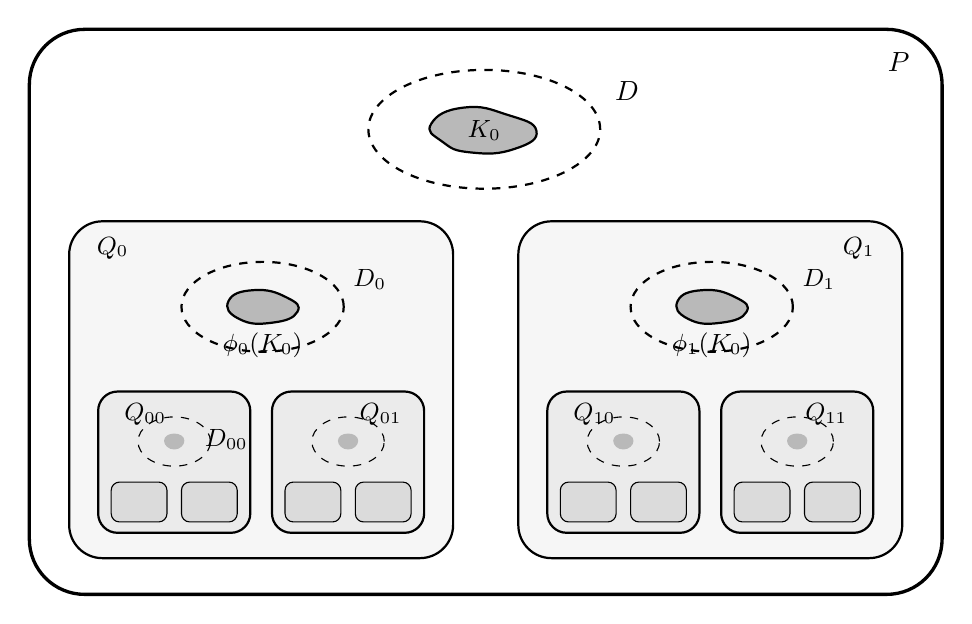
\begin{tikzpicture}[scale=0.92, line join=round, font=\small]
% ---------- the piece P ----------
\draw[very thick, rounded corners=20pt] (0,0) rectangle (12.6,7.8);
\node[font=\normalsize] at (12.0,7.35) {$P$};
% ---------- first-level pullbacks Q_0, Q_1 ----------
\draw[thick, fill=gray!7, rounded corners=12pt] (0.55,0.5) rectangle (5.85,5.15);
\draw[thick, fill=gray!7, rounded corners=12pt] (6.75,0.5) rectangle (12.05,5.15);
\node at (1.15,4.78) {$Q_0$};
\node at (11.45,4.78) {$Q_1$};
% ---------- second-level cylinders inside Q_0 ----------
\draw[thick, fill=gray!16, rounded corners=7pt] (0.95,0.85) rectangle (3.05,2.8);
\draw[thick, fill=gray!16, rounded corners=7pt] (3.35,0.85) rectangle (5.45,2.8);
\node at (1.6,2.48) {$Q_{00}$};
\node at (4.85,2.48) {$Q_{01}$};
% ---------- second-level cylinders inside Q_1 ----------
\draw[thick, fill=gray!16, rounded corners=7pt] (7.15,0.85) rectangle (9.25,2.8);
\draw[thick, fill=gray!16, rounded corners=7pt] (9.55,0.85) rectangle (11.65,2.8);
\node at (7.8,2.48) {$Q_{10}$};
\node at (11.0,2.48) {$Q_{11}$};
% ---------- third-level cylinders (unlabeled) and tiny fibers inside Q_00 ----------
\draw[fill=gray!28, rounded corners=3pt] (1.13,1.0) rectangle (1.9,1.55);
\draw[fill=gray!28, rounded corners=3pt] (2.1,1.0) rectangle (2.87,1.55);
\fill[gray!55] plot [smooth cycle, tension=1] coordinates
  {(1.86,2.12) (2.0,2.22) (2.14,2.12) (2.0,2.0)};
\draw[dashed] (2.0,2.11) ellipse (0.5 and 0.34);
\node at (2.72,2.14) {$D_{00}$};
% ---------- third-level cylinders and tiny fibers inside Q_01 ----------
\draw[fill=gray!28, rounded corners=3pt] (3.53,1.0) rectangle (4.3,1.55);
\draw[fill=gray!28, rounded corners=3pt] (4.5,1.0) rectangle (5.27,1.55);
\fill[gray!55] plot [smooth cycle, tension=1] coordinates
  {(4.26,2.12) (4.4,2.22) (4.54,2.12) (4.4,2.0)};
\draw[dashed] (4.4,2.11) ellipse (0.5 and 0.34);
% ---------- third-level cylinders and tiny fibers inside Q_10 ----------
\draw[fill=gray!28, rounded corners=3pt] (7.33,1.0) rectangle (8.1,1.55);
\draw[fill=gray!28, rounded corners=3pt] (8.3,1.0) rectangle (9.07,1.55);
\fill[gray!55] plot [smooth cycle, tension=1] coordinates
  {(8.06,2.12) (8.2,2.22) (8.34,2.12) (8.2,2.0)};
\draw[dashed] (8.2,2.11) ellipse (0.5 and 0.34);
% ---------- third-level cylinders and tiny fibers inside Q_11 ----------
\draw[fill=gray!28, rounded corners=3pt] (9.73,1.0) rectangle (10.5,1.55);
\draw[fill=gray!28, rounded corners=3pt] (10.7,1.0) rectangle (11.47,1.55);
\fill[gray!55] plot [smooth cycle, tension=1] coordinates
  {(10.46,2.12) (10.6,2.22) (10.74,2.12) (10.6,2.0)};
\draw[dashed] (10.6,2.11) ellipse (0.5 and 0.34);
% ---------- root gap: K_0 and its cell D ----------
\fill[gray!55] plot [smooth cycle, tension=0.9] coordinates
  {(5.55,6.5) (6.0,6.72) (6.6,6.62) (7.0,6.4) (6.7,6.15) (6.1,6.1) (5.7,6.25)};
\draw[thick] plot [smooth cycle, tension=0.9] coordinates
  {(5.55,6.5) (6.0,6.72) (6.6,6.62) (7.0,6.4) (6.7,6.15) (6.1,6.1) (5.7,6.25)};
\node at (6.28,6.4) {$K_0$};
\draw[dashed, thick] (6.28,6.42) ellipse (1.6 and 0.82);
\node[font=\normalsize] at (8.25,6.95) {$D$};
% ---------- level-1 gap of Q_0 ----------
\fill[gray!55] plot [smooth cycle, tension=0.9] coordinates
  {(2.75,4.05) (3.1,4.2) (3.55,4.1) (3.7,3.9) (3.35,3.75) (2.9,3.8)};
\draw[thick] plot [smooth cycle, tension=0.9] coordinates
  {(2.75,4.05) (3.1,4.2) (3.55,4.1) (3.7,3.9) (3.35,3.75) (2.9,3.8)};
\node[below=1pt] at (3.22,3.78) {$\phi_0(K_0)$};
\draw[dashed, thick] (3.22,3.97) ellipse (1.12 and 0.62);
\node at (4.7,4.35) {$D_0$};
% ---------- level-1 gap of Q_1 ----------
\fill[gray!55] plot [smooth cycle, tension=0.9] coordinates
  {(8.95,4.05) (9.3,4.2) (9.75,4.1) (9.9,3.9) (9.55,3.75) (9.1,3.8)};
\draw[thick] plot [smooth cycle, tension=0.9] coordinates
  {(8.95,4.05) (9.3,4.2) (9.75,4.1) (9.9,3.9) (9.55,3.75) (9.1,3.8)};
\node[below=1pt] at (9.42,3.78) {$\phi_1(K_0)$};
\draw[dashed, thick] (9.42,3.97) ellipse (1.12 and 0.62);
\node at (10.9,4.35) {$D_1$};
\end{tikzpicture}
\caption{The direct-decoration gap-cell atlas through depth two.  The
closed Jordan piece $P$ contains the two disjoint closed univalent
pullbacks $Q_0$ and $Q_1$, each of which contains its own next-level
cylinders $Q_{a0},Q_{a1}$, and so on.  The root continuum $K_0$ (blob)
lies in the root gap $P\setminus(Q_0\cup Q_1)$, and the dashed closed
Jordan cell $D$ supplied by Lemma~\ref{lem:jordan-nbhd} isolates it:
$K_0\subset\Int D\subset D\Subset\Int P\setminus(Q_0\cup Q_1)$.  The
inverse branches transport the picture into every cylinder: the fiber
$K_w=\phi_w(K_0)$ lies in the gap of its own cylinder $Q_w$, surrounded
by the dashed cell $D_w=\phi_w(D)\Subset\Int Q_w\setminus(Q_{w0}\cup
Q_{w1})$; the depth-one and depth-two cells $D_0$, $D_1$, $D_{00}$,
$\dots$ are shown.  The cells are pairwise disjoint, including for
ancestor--descendant words, and each one isolates its fiber from the
entire rooted-end compactum: $D_w\cap H_\partial=K_w$
(Theorem~\ref{thm:gap-cells}), so every unselected finite fiber and
every end fiber misses $D_w$.  Dynamics transports the atlas by
$g(D_{aw})=D_w$.}
\label{fig:cells}
\end{figure}

The atlas should be compared clause for clause with
Proposition~\ref{prop:cellwise}: the cells $D_w$ are the pairwise
disjoint closed Jordan disks demanded there, the fibers $K_w$ are the
raw seeds, the fill containment \eqref{eq:F-cell-fill} is the
localization clause, and the exit arcs will be supplied by
Lemma~\ref{lem:impression-port} below.  What the dynamics adds to the
static cellwise picture is the isolation identity
$D_w\cap H_\partial=K_w$, which controls not only the finitely many
packets that a certificate names but \emph{all} fibers of the infinite
compactum at once, and the transport identity $g(D_{aw})=D_w$, which
makes the atlas equivariant.

\subsection{Packet replacement}\label{subsec:F-replacement}

An augmented packet replaces an atom by the filled hull of the atom
together with its protected collars.  In the decoration setting the atoms
are finite fibers, and the replacement must not disturb the connected
complement guaranteed by Theorem~\ref{thm:full-fibers}---otherwise the
free-component criterion of Theorem~\ref{thm:free-component} could fail
after fullification for reasons invisible in the certificate.  The next
theorem rules this out: fullifying finitely many selected fibers inside
their cells leaves the complement connected.

\begin{theorem}[Finite direct-decoration packet replacement; manuscript
Theorem 10.43]\label{thm:packet-replacement}
Let $F\subset\mathcal A^{<\mathbb N}$ be finite and let
\begin{equation}\label{eq:F-replacement}
K_w\subset L_w\Subset\Int D_w,\qquad w\in F,
\end{equation}
with every $L_w$ full (display (DG6) of \cite{MWman}).  Then replacing
the selected fibers $K_w$ by $L_w$ in $H_\partial$, that is, forming
\[
H'
=\Bigl(H_\partial\setminus\bigcup_{w\in F}K_w\Bigr)
\cup\bigcup_{w\in F}L_w ,
\]
gives a compact set with connected sphere complement.
\end{theorem}

\begin{proof}
\emph{The replacement is compact.}
The isolation identity \eqref{eq:F-cell-isolation} makes each selected
$K_w$ clopen in $H_\partial$: it is relatively closed because
$K_w=D_w\cap H_\partial$ with $D_w$ closed, and relatively open because
$K_w=\Int D_w\cap H_\partial$ by \eqref{eq:F-cell-position} and the same
identity.  Hence $H_\partial\setminus\bigcup_{w\in F}K_w$ is a relatively
closed subset of the compact set $H_\partial$, so it is compact, and its
union $H'$ with the finitely many compacta $L_w$ is compact.

\emph{Cells meet deep approximants only in their fibers.}
Fix $w\in F$ and let $m>|w|$.  We claim
\begin{equation}\label{eq:F-cell-approximants}
D_w\cap H_m=K_w ,
\end{equation}
where $H_m$ is the approximant \eqref{eq:F-approximants}.  The inclusion
$\supset$ holds because $K_w$ is a term of $H_m$ (as $|w|<m$) and
$K_w\subset D_w$.  For $\subset$, run the dichotomy of the proof of
Theorem~\ref{thm:gap-cells} over the terms of $H_m$.  A fiber term $K_u$,
$|u|<m$, $u\ne w$: incomparable words have disjoint cylinders; if $u$ is
a strict prefix of $w$ then $D_w\subset Q_{ua}$ for the appropriate child
while \eqref{eq:F-root-gap-pullback} keeps $K_u$ out of both children; if
$w$ is a strict prefix of $u$ then $K_u\subset Q_{wa}$ for some
$a\in\mathcal A$, while $D_w$ misses both children of $Q_w$ by
\eqref{eq:F-cell-position}.  A cylinder term $Q_v$, $|v|=m>|w|$: if $v$
and $w$ are incomparable their cylinders are disjoint; otherwise $w$ is a
strict prefix of $v$, so $Q_v\subset Q_{wa}$ for some $a$, which $D_w$
misses.  This proves \eqref{eq:F-cell-approximants}.

\emph{Modified approximants.}
Put $M=\max_{w\in F}|w|$ and, for $m>M$, make the same replacements in
the approximants:
\[
H_m'
=\Bigl(H_m\setminus\bigcup_{w\in F}K_w\Bigr)
\cup\bigcup_{w\in F}L_w .
\]
Each $H_m'$ is again a finite union of pairwise disjoint full continua.
Indeed, the terms of $H_m$ other than the selected fibers are unchanged,
and each selected term $K_w$ is replaced by the full continuum $L_w$;
disjointness survives because, by \eqref{eq:F-cell-approximants},
\[
L_w\subset\Int D_w
\quad\text{and}\quad
D_w\cap H_m=K_w ,
\]
so $L_w$ meets no unselected term of $H_m$, and distinct selected
replacements $L_w,L_{w'}$ lie in the disjoint cells $D_w,D_{w'}$ of
Theorem~\ref{thm:gap-cells}.  The modified approximants decrease: the
unreplaced parts decrease as in the proof of
Theorem~\ref{thm:full-fibers}, and the replaced terms $L_w$ are constant
in $m$.  Their intersection is the modified rooted-end compactum:
\[
\bigcap_{m>M}H_m'
=\Bigl(\bigcap_{m>M}H_m\setminus\bigcup_{w\in F}K_w\Bigr)
\cup\bigcup_{w\in F}L_w
=H' ,
\]
where the first equality uses \eqref{eq:F-cell-approximants} twice: a
point of $D_w$ lies in $H_m'$ exactly when it lies in $L_w$, and a point
outside every selected cell lies in $H_m'$ exactly when it lies in
$H_m$.

\emph{Conclusion.}
The sets $H_m'$, $m>M$, form a decreasing sequence of compact sets, each
a finite union of pairwise disjoint full continua, with intersection
$H'$.  Lemma~\ref{lem:nested-packets} shows that $\Chat\setminus H'$ is
connected.
\end{proof}

\begin{remark}\label{rem:F-localized}
The proof yields a localized supplement that Theorem~\ref{thm:carrier}
uses.  Fix any Jordan domain $U$ with $P\Subset U$---for instance a
round disk containing $P$.  Every approximant, modified or not, lies in
$P$, hence is compactly contained in $U$, so the localized clause of
Lemma~\ref{lem:nested-packets} applies to the sequence $(H_m')_{m>M}$
and shows that $U\setminus H'$ is connected: the replaced compactum has
one \emph{common} complementary component inside the localization, not
merely a connected complement on the sphere.
\end{remark}

\subsection{Ports at proper protected impressions}\label{subsec:F-port}

The free-component criterion requires each atom to retain a free
singleton port not equal to a protected impression.  In the decoration
setting the atom is a fiber $K_w$, the protected data are finitely many
prime-end crosscut chains, and the port must avoid not only the chains'
collars but the entire fullification of the fiber together with those
collars.  The next lemma produces such a port from a purely metric
selection, under the sole hypothesis that the protected impressions do
not exhaust the boundary.

\begin{lemma}[Proper protected impressions leave a port; manuscript
Lemma 10.44]\label{lem:impression-port}
Let $K\Subset\Int D$ be a nondegenerate full continuum in a closed
Jordan disk $D$, and let $P_{\mathrm{prot}}\subsetneq\partial K$ be
compact.  Then there are a point
$x\in\partial K\setminus P_{\mathrm{prot}}$ and a Jordan arc $\alpha$
from $x$ to $\partial D$, otherwise in $\Int D\setminus K$.  Moreover,
finitely many protected crosscut-chain collars whose impressions have
union contained in $P_{\mathrm{prot}}$ can be truncated so that, for the
connected union $S$ of $K$ with the truncated closed collars,
\begin{equation}\label{eq:F-port}
\alpha\cap\Fill(S)=\{x\}
\end{equation}
(display (DG7) of \cite{MWman}).
\end{lemma}

\begin{proof}
\emph{Metric selection of the port point.}
Since $P_{\mathrm{prot}}$ is a proper compact subset of $\partial K$,
choose $y\in\partial K\setminus P_{\mathrm{prot}}$ and put
$\delta=\dist(y,P_{\mathrm{prot}})>0$ (with $\delta=+\infty$ if
$P_{\mathrm{prot}}=\varnothing$).  Because $y$ is a boundary point of $K$
and $K\Subset\Int D$, every small ball around $y$ contains points of
$\Int D\setminus K$; choose
\[
z\in\Int D\setminus K,\qquad |z-y|<\delta/4 .
\]
Let $x\in K$ minimize the distance to $z$; the minimum is positive since
$z\notin K$ and $K$ is compact.  Every point $p$ of the half-open segment
$(x,z]$ satisfies $|p-z|<|x-z|=\dist(z,K)$, so $(x,z]$ misses $K$; in
particular $x$ is a limit of points of the complement, so
$x\in\partial K$.  The triangle inequality and the minimizing property
(applied against the competitor $y\in K$) give
\[
|x-y|\le|x-z|+|z-y|\le 2|z-y|<\delta/2 ,
\]
hence
$\dist(x,P_{\mathrm{prot}})\ge\delta-|x-y|>\delta/2$ and
$x\notin P_{\mathrm{prot}}$.

\emph{Construction of the arc.}
The complement $\C\setminus K$ of the full continuum is an open connected
subset of the plane, hence arcwise connected \cite{New51}.  Join $z$ by
an arc in $\C\setminus K$ to some point outside $D$, and concatenate
with the segment from $x$ to $z$.  The concatenation is a path from $x$
leaving $D$, contained in $(\C\setminus K)\cup\{x\}$ and meeting $K$ only
at its initial point; extract from it a Jordan arc from $x$ to the far
endpoint, which again meets $K$ only at $x$.  Since the arc starts in
$\Int D$ and ends outside $D$, the parameter set of points on $\partial
D$ is nonempty and closed; truncating at the \emph{first hit} on
$\partial D$ yields a Jordan arc $\alpha$ from $x$ to a point of
$\partial D$ with $\alpha\setminus\{x,\alpha(1)\}\subset\Int D$ and
$\alpha\cap K=\{x\}$.  This proves the first assertion.

\emph{Truncation of the collars.}
Let the finitely many protected chains be
$(\gamma_{j,n},D_{j,n})_{n\ge1}$, prime-end crosscut chains of
$\Chat\setminus K$ whose impressions
$I_j=\bigcap_n\overline{D_{j,n}}$ satisfy
$\bigcup_jI_j\subset P_{\mathrm{prot}}$.  Since $\alpha\cap K=\{x\}$ and
$x\notin P_{\mathrm{prot}}$, the compact sets $\alpha$ and
$P_{\mathrm{prot}}$ are disjoint and have positive distance $2\rho>0$.
Shrinking $\rho$ if necessary, choose for each $j$ an open neighborhood
$W_j$ of $I_j$ contained in the $\rho$-neighborhood of
$P_{\mathrm{prot}}$, in $\Int D$ (possible since
$I_j\subset\partial K\subset K\Subset\Int D$), and in the prescribed
neighborhood of $I_j$ if one was given.  The closures
$\overline{D_{j,n}}$ are nested compact sets with intersection $I_j$, so
for every $j$ there is $n_j$ with
$\overline{D_{j,n_j}}\subset W_j$: otherwise compactness would place a
point of $\bigcap_n\overline{D_{j,n}}=I_j$ outside $W_j$.  Truncate the
$j$-th chain at depth $n_j$ and set
\[
S=K\cup\bigcup_j\overline{D_{j,n_j}} .
\]
Each closed collar meets $K$ in its nonempty impression
$I_j\subset\overline{D_{j,n_j}}\cap K$, so $S$ is a compact connected
set, and $S\Subset\Int D$ by the choice of the $W_j$.  By construction
the truncated collars lie in the $\rho$-neighborhood of
$P_{\mathrm{prot}}$ and therefore miss $\alpha$; hence
\[
\alpha\cap S=\alpha\cap K=\{x\}.
\]

\emph{Extension to infinity and \eqref{eq:F-port}.}
Extend $\alpha$ beyond its endpoint on $\partial D$ by an arc to
$\infty$ in $\C\setminus\Int D$ (for instance, along the image of a
radial ray of the exterior of $D$).  The set
\[
\beta=\alpha\bigl((0,1]\bigr)\cup(\text{the extension})
\]
is connected and unbounded and misses $S$: the extension misses
$S\Subset\Int D$, and $\alpha((0,1])$ misses $S$ by the previous step.
Hence $\beta$ lies in the unbounded component of $\C\setminus S$, and no
point of $\beta$ belongs to $\Fill(S)$, which is $S$ together with the
\emph{bounded} complementary components.  Every point of $\alpha$ except
$x$ lies in $\beta$, and $x\in K\subset S\subset\Fill(S)$; therefore
$\alpha\cap\Fill(S)=\{x\}$, which is \eqref{eq:F-port}.
\end{proof}

\begin{remark}\label{rem:F-collar-confinement}
The proof gives slightly more than the statement: the truncation can
confine the truncated closed collars to any prescribed open
neighborhoods of their impressions, since nested compact crosscut-chain
closures have intersection equal to their impressions and sufficiently
deep tails therefore lie in any such neighborhoods.  This supplement is
established by the proof above, following the manuscript's own proof of
Lemma 10.44; the manuscript's printed statement ends at
\eqref{eq:F-port}, and we use the supplement below with this explicit
attribution.
\end{remark}

\subsection{The protected-carrier theorem}\label{subsec:F-carrier}

The pieces are now assembled.  The theorem below is the finite,
checkable statement toward which the whole paper has been building: at
any fixed decoration depth, any finite selection of fibers, decorated by
actual protected prime-end chains at the root whose impressions do not
exhaust the root boundary, is joined by a protected regulated connector
that respects every piece of the frozen inventory---including the
infinitely many unselected fibers and end fibers.

\begin{theorem}[Finite direct-decoration protected carrier; manuscript
Theorem 10.45]\label{thm:carrier}
Fix a finite set $F\subset\mathcal A^{<\mathbb N}$ of direct-decoration
addresses, and fix finitely many actual protected prime-end crosscut
chains of $\Chat\setminus K_0$ at the root whose total impression is a
proper compact subset of $\partial K_0$.  Then sufficiently deep collar tails of the protected
chains, and the free port supplied by
Lemma~\ref{lem:impression-port}, can be transported through the inverse
branches $\phi_w$, $w\in F$, so that the resulting packet fullifications
remain in the pairwise disjoint cells $D_w$, avoid every unselected
finite fiber and every end fiber, and admit a protected regulated
connector preserving the transported prime ends and their cyclic order.
\end{theorem}

\begin{proof}
\emph{Step 1: root data.}
Discarding duplicates, assume the given chains define pairwise distinct
prime ends: two equivalent chains protect the same access, so nothing is
lost.  Apply Lemma~\ref{lem:impression-port} with $K=K_0$, with $D$ the root
cell of the atlas construction (so $K_0\Subset\Int D$ by
\eqref{eq:F-cell-position} at the empty word), and with
$P_{\mathrm{prot}}$ the union of the impressions of the given protected
chains---a finite union of compacta, compact, and a proper subset of
$\partial K_0$ by hypothesis.  The lemma yields a port point
$x\in\partial K_0\setminus P_{\mathrm{prot}}$, a Jordan arc $\alpha$ from
$x$ to $\partial D$ meeting $K_0$ only at $x$, and truncations of the
protected chains, with closed collar tails in prescribed neighborhoods of
their impressions (Remark~\ref{rem:F-collar-confinement}), such that the
connected union $S$ of $K_0$ with the
truncated closed collars satisfies $S\Subset\Int D$ and
$\alpha\cap\Fill(S)=\{x\}$.  Because the chains define pairwise distinct
prime ends, their deep selected domains are eventually pairwise
disjoint, so after a further truncation---which keeps every conclusion,
the deeper collars being nested in the previous ones---the closed collar
tails may in addition be taken pairwise disjoint, exactly as in the
truncation normalization of Section~\ref{sec:certificates}.  By the fill
containment \eqref{eq:F-cell-fill} applied at the empty word,
\[
\Fill(S)\Subset\Int D .
\]

\emph{Step 2: transport through the inverse branches.}
For $w\in F$ let $\Phi_w\colon\Chat\to\Chat$ be the orientation-preserving
sphere extension of $\phi_w$ constructed in the proof of
Theorem~\ref{thm:full-fibers}.  Define the transported data at address
$w$:
\[
S_w=\Phi_w(S),\qquad
\alpha_w=\Phi_w(\alpha),\qquad
x_w=\phi_w(x),
\]
together with the transported protected chains
$\Phi_w(\gamma_{j,n},D_{j,n})_{n\ge n_j}$.  As in the proof of
Proposition~\ref{prop:naturality}, an orientation-preserving sphere
homeomorphism carries crosscuts of $\Chat\setminus K_0$ to crosscuts of
$\Chat\setminus K_w$, null chains to null chains, selected sides to
selected sides, and preserves the cyclic order of prime ends; so the
transported chains are prime-end crosscut chains of
$\Chat\setminus K_w$, pairwise distinct, with impressions
$\Phi_w(I_j)\subset\partial K_w$, and $S_w$ is the connected union of
$K_w$ with their truncated closed collars.  Fullification commutes with
the transport: $\Phi_w$ maps $\Chat\setminus P$ onto
$\Chat\setminus Q_w$, hence maps the complementary component of $S$
containing $\Chat\setminus P$---the unbounded one---onto the
complementary component of $S_w$ containing $\Chat\setminus Q_w$---again
the unbounded one---and maps the remaining (bounded) complementary
components bijectively onto the remaining ones; therefore
\[
L_w:=\Fill(S_w)=\Phi_w\bigl(\Fill(S)\bigr).
\]
Applying $\Phi_w$ to the Step-1 inclusions and to \eqref{eq:F-port}
gives
\[
K_w\subset L_w\Subset\Int D_w,
\qquad
\alpha_w\cap L_w=\{x_w\},
\]
with $\alpha_w$ a Jordan arc from $x_w$ to $\partial D_w$, otherwise in
$\Int D_w\setminus K_w$.  Each $L_w$ is full: the filled hull of a
continuum is a full continuum.

\emph{Step 3: localization and isolation.}
Theorem~\ref{thm:gap-cells} now localizes and isolates the packets.  The
cells $D_w$, $w\in F$, are pairwise disjoint, so the packet
fullifications $L_w\subset D_w$ are pairwise disjoint and each port arc
$\alpha_w\subset D_w$ meets every other packet's cell not at all.  By the
isolation identity \eqref{eq:F-cell-isolation}, every component of
$H_\partial$ other than $K_w$ misses $D_w$; hence every $L_w$, and every
$\alpha_w$, avoids every unselected finite fiber and every end fiber.

\emph{Step 4: one common free component after fullification.}
The data \eqref{eq:F-replacement} of
Theorem~\ref{thm:packet-replacement} hold for the family
$(L_w)_{w\in F}$, so the replaced compactum
\[
H'=\Bigl(H_\partial\setminus\bigcup_{w\in F}K_w\Bigr)
\cup\bigcup_{w\in F}L_w
\]
is compact with connected sphere complement; and by
Remark~\ref{rem:F-localized}, for a fixed Jordan localization $U$ with
$P\Subset U$ the set $U\setminus H'$ is connected.  Freeze the
inventory of Section~\ref{sec:criterion} as follows: the original atoms
are the selected fibers $K_w$; the closed terminal protected collars are
the truncated collar tails, absorbed into the completed packets $L_w$;
the obstacles are the unselected finite fibers and the end fibers, that
is, $H_\partial\setminus\bigcup_{w\in F}K_w$; the critical-value
exclusion is empty, the branch system \eqref{eq:F-pullbacks} being
univalent; and the localization-forbidden set is $\Chat\setminus U$.
The raw frozen set $Q$ of Section~\ref{sec:criterion} consists of the
listed pieces themselves; the completed packets $L_w$ enlarge the
selected atoms with their truncated collars and the bounded
complementary components added by $\Fill$.  The set $U\setminus H'$ is
connected by Remark~\ref{rem:F-localized}, it lies in
$\Omfree=U\setminus Q$ because $H'\supset Q\cap U$, and it is in fact an
entire component $\Omega_0$ of $\Omfree$: its relative boundary in $U$
lies in $H'$, while the finitely many fill components of the packets
$L_w\setminus S_w$, the only points of $H'$ not in $Q$, are open subsets
of $U\setminus Q$ separate from $U\setminus H'$.  So the component
$\Omega_0=U\setminus H'$ of the frozen free domain contains every port
interior, as the next paragraph verifies.

The port arcs land in it.  Fix $w\in F$.  The cell identity
$D_w\cap H_\partial=K_w$ and the disjointness of the cells give
$D_w\cap H'=L_w$, and $\alpha_w\cap L_w=\{x_w\}=\{\alpha_w(0)\}$; since
$\alpha_w\subset D_w\subset U$, the half-open arc
$\alpha_w((0,1])$ lies in $U\setminus H'=\Omega_0$.  The arcs
$\alpha_w$, $w\in F$, are pairwise disjoint, lying in pairwise disjoint
cells.  Thus $\Omega_0$ has simultaneous singleton ports to every
required atom $K_w$, with each port point $x_w$ a free point not equal
to a protected impression
($x\notin P_{\mathrm{prot}}$ transports to
$x_w\notin\Phi_w(P_{\mathrm{prot}})$).

\emph{Step 5: conclusion by the criterion and the realization theorem.}
By Theorem~\ref{thm:free-component}, the frozen data admit a protected
ribbon-routing certificate: the single free component $\Omega_0$ has
simultaneous singleton ports to every required atom.
Theorem~\ref{thm:realization} realizes the certificate by a compact
connected full carrier that contains every selected fiber $K_w$, has
singleton attachment trace $\{x_w\}$ at each, misses the frozen obstacle
set---in particular every unselected finite fiber and every end
fiber---and preserves every transported protected chain as a prime-end
chain of the enlarged complement, with injective survival and unchanged
cyclic order.  The cyclic order in question is the transported one: by
Step 2 the transport $\Phi_w$ is orientation-preserving and carries the
root cyclic order of the protected chains to the cyclic order at $K_w$,
and Theorem~\ref{thm:realization}(4) preserves the latter.  This is the
asserted protected regulated connector.
\end{proof}

We reproduce the manuscript's caveat, recorded immediately after
Theorem~10.45 of \cite{MWman}, in its own warning environment; the Scope
section returns to it.

\begin{warning}\label{warn:F-finite-scale}
The protected-carrier theorem, Theorem~\ref{thm:carrier}, is finite and
direct-scale only.  It does not construct a second satellite portrait, an
end-fiber return map, a uniform incidence bound, or future fjord, dam,
and attachment data.
\end{warning}

This section is the framework's intended mode of use, and it is worth
stating plainly what has and has not been done.  What has been done is
finite and checkable: at a fixed decoration depth, for an explicitly
listed selection of addresses and an explicitly listed family of
protected root accesses, Theorem~\ref{thm:carrier} produces a protected
regulated connector whose every property---localization in the cells,
isolation from the unselected and end fibers, survival and cyclic order
of the protected prime ends---is certified by the finite data of the
gap-cell atlas and the packet audit, and each such certificate persists
under the monotone operations of Section~\ref{sec:audit}.  What has not
been done is everything infinite or virtual.  The manuscript's open
problems 10.50 (the virtual cylinder target-address selector), 10.51
(disconnected marking transfer to actual bases and iterates on the
cylinders and end fibers of Theorem~\ref{thm:F-compactification}), and
10.52 (virtual Cantor-package realization at every intermediate scale)
are stated as open in \cite{MWman}, remain open, and are not advanced by
anything in this section: no return map on end fibers is constructed, no
end fiber is identified with a small Julia set, and no selection of
target addresses for virtual cylinders is made.  The finite theorem is
offered as what it is---a template showing that, whenever the missing
virtual data are someday supplied, the planar routing they require is
already exact, certified, and persistent.

